% chapters/chapter1/sec4.tex

\section{先修知识梳理：数字通信核心原理、雷达感知核心原理}
\label{sec:ch1-prerequisites}
 

\subsection{本节设置目的}
\label{subsec:ch1-prerequisites-purpose}

% TODO:
% 1. 说明为什么需要先修知识梳理；
% 2. 明确本节的定位边界；
% 3. 说明本节和后续 ISAC 章节的关系。

正文待补充。

\subsection{数字通信核心原理梳理}
\label{subsec:ch1-digital-comm}


 
\noindent\textbf{数字通信系统的基本链路}


在数字通信系统中，信息传输并不是简单地将信号从发射端送到接收端，
而是一个围绕“比特可靠恢复”展开的系统化过程。
发射端首先将待传输的信息转化为适合无线信道传播的电磁信号，
接收端则需要在噪声、衰落、多径和干扰等不利条件下，
从接收信号中尽可能准确地恢复原始信息比特。
因此，从通信角度看，系统设计的核心目标可以概括为：
在有限带宽、有限功率和复杂无线环境中，实现高可靠、高效率的信息传输。

这一基本链路也是理解 ISAC 的起点。
ISAC 并不是脱离通信系统重新构造一套独立的感知系统，
而是在已有通信链路的基础上进一步挖掘无线信号的感知能力。
也就是说，同一个发射信号既可以承载通信比特，
也可能通过传播、反射和接收过程携带环境或目标信息。
因此，在讨论 ISAC 之前，有必要先明确数字通信链路的基本组成，
以及这些组成部分如何为后续的联合波形设计、信道建模、
MIMO 波束成形和资源优化奠定基础。

图~\ref{fig:communication_chain} 给出了一个典型数字通信系统的基本框图。
该框图并不旨在完整展开通信系统的全部细节，
而是帮助读者建立一个最小必要的链路认知：
信息比特如何被转换为无线信号，
信号如何经过信道传播，
接收端又如何从受损信号中恢复信息。
\begin{figure}[htbp]
    \centering
    \begin{tikzpicture}[
        % 调整全局间距：拉开横向距离以容纳文字标签，纵向保持紧凑
        node distance=1.8cm and 1.5cm,
        % 定义方框样式
        block/.style={
            rectangle,
            draw=black,
            thick,
            fill=white,
            minimum width=2.2cm,
            minimum height=1.2cm,
            text centered,
            font=\sffamily\large
        },
        % 定义箭头样式
        arrow/.style={
            ->,
            >=Stealth,
            thick
        },
        % 定义标签文字样式 
        label_text/.style={
            font=\sffamily\small,
            color=black
        }
    ]

    % 1. 发射端节点 (从左到右)
    \node[block] (source) {信源};
    \node[block, right=of source] (src_enc) {信源编码};
    \node[block, right=of src_enc] (chn_enc) {信道编码};
    \node[block, right=of chn_enc] (mod) {调制};

    % 发射端虚线框及标签
    \node[draw, dashed, thick, inner sep=14pt, fit=(source) (mod)] (tx_box) {};
    \node[above=0.2cm of tx_box.north, font=\sffamily\Large\bfseries] {发射端};

    % 2. 无线信道 (在调制的正下方)
    \node[block, below=1.8cm of mod] (channel) {无线信道};
    
    % 噪声注入
    \node[left=1.5cm of channel] (noise) {噪声/干扰};
    \draw[arrow, dashed, gray] (noise) -- (channel);

    % 3. 接收端节点 (从右到左，完美对齐上方)
    \node[block, below=1.8cm of channel] (recv) {接收};
    \node[block, left=of recv] (demod) {解调};
    \node[block, left=of demod] (dec) {译码};
    \node[block, left=of dec] (sink) {信宿}; 

    % 接收端虚线框及标签
    \node[draw, dashed, thick, inner sep=14pt, fit=(recv) (sink)] (rx_box) {};
    \node[below=0.2cm of rx_box.south, font=\sffamily\Large\bfseries] {接收端};

    % 4. 绘制连线与信号状态标注
    \draw[arrow] (source) -- node[above, label_text] {原始信息} (src_enc);
    \draw[arrow] (src_enc) -- node[above, label_text] {信息比特} (chn_enc);
    \draw[arrow] (chn_enc) -- (mod);
    
    \draw[arrow] (mod) -- node[right, label_text] {射频信号} (channel);
    \draw[arrow] (channel) -- node[right, label_text] {受损信号} (recv);
    
    \draw[arrow] (recv) -- (demod);
    \draw[arrow] (demod) -- node[above, label_text] {译码比特} (dec);
    \draw[arrow] (dec) -- (sink); 

    \end{tikzpicture}
    \caption{数字通信系统基本链路框图}
    \label{fig:communication_chain}
\end{figure}
\begin{itemize}
    \item \textbf{信源：}
    信源产生待传输的原始信息。
    在数字通信系统中，这些信息通常可以抽象为原始比特序列。
    例如，文本、语音、图像或传感数据在进入通信系统后，
    都需要被表示为离散的数字比特。

    \item \textbf{信源编码：}
    信源编码的主要作用是压缩信息中的冗余，
    提高信息表达效率。
    经过信源编码后，原始信息被转换为更加紧凑的信息比特流，
    以减少后续传输所需的资源开销。

    \item \textbf{信道编码：}
    信道编码的主要作用是增强通信系统的可靠性。
    它通过向信息比特中引入受控冗余，
    使接收端能够在噪声、衰落和干扰存在的情况下，
    检测并纠正一定程度的传输错误。
    因此，信道编码后的比特也常被称为编码比特。

    \item \textbf{调制：}
    调制的作用是将离散的编码比特映射为适合无线传输的调制符号，
    并进一步形成射频信号进行发射。
    常见调制方式包括 PSK、QAM 等。
    在 ISAC 系统中，调制波形不仅影响通信数据的传输效率，
    也会影响感知任务中的距离、速度和角度估计能力。

    \item \textbf{无线信道：}
    无线信道描述射频信号在空间传播过程中的变化。
    信号在传播时会受到路径损耗、多径衰落、噪声和干扰等因素影响。
    因此，接收端获得的信号是经过信道畸变并叠加噪声后的受损信号。
    对于 ISAC 而言，无线信道不仅影响通信质量，
    也携带了与环境、目标和传播路径相关的感知信息。

    \item \textbf{接收：}
    接收模块负责从无线信道中获取受信号，
    并完成下变频、采样、同步等前端处理。
    接收信号中同时包含有用信号、噪声、干扰以及信道传播效应。
    在 ISAC 系统中，接收信号还可能包含由目标或环境反射产生的回波信息。

    \item \textbf{解调：}
    解调的作用是根据接收信号估计发送端的调制符号，
    并进一步得到对应的软信息或判决比特。
    由于信号在无线信道中受到噪声和干扰影响，
    解调结果可能存在误判，因此后续仍需要依赖信道译码进一步提高可靠性。

    \item \textbf{译码：}
    译码模块根据发送端采用的信道编码规则，
    利用解调输出的软信息或判决比特恢复原始信息比特。
    译码过程的目标是尽可能纠正传输过程中产生的错误，
    使接收端恢复的信息尽可能接近发送端的信息。

    \item \textbf{信宿：}
    信宿是信息传输的最终目的端。
    它接收译码后恢复出的信息，
    并将其用于后续的数据处理、显示、存储或控制任务。
\end{itemize}
从 ISAC 的角度看，最值得关注的是调制波形、无线信道、
天线阵列和接收信号处理等环节。
因为感知功能通常并不直接作用于“比特”本身，
而是利用无线信号在传播和反射过程中携带的环境信息。
例如，发射波形决定了距离和速度分辨能力，
信道响应包含目标或环境的空间特征，
接收信号处理则决定了系统能否在恢复通信信息的同时提取感知参数。
因此，数字通信链路不仅是信息传输的基础，
也是 ISAC 实现通信与感知融合的物理载体。


\paragraph{通信系统的基本信号模型}

在通信系统中，发射信号经过无线信道后会发生衰落、多径扩展，
并叠加噪声或干扰。
其时域基带模型可表示为
\begin{equation}
    y(t) = h(t) * x(t) + n(t),
    \label{eq:comm_time_domain_model}
\end{equation}
其中，\(x(t)\) 为发射基带信号，
\(h(t)\) 为无线信道冲激响应，
\(n(t)\) 为噪声或干扰，
\(y(t)\) 为接收信号，
\(*\) 表示卷积运算。
该模型表明，接收端观测到的信号是信号、信道和噪声共同作用的结果。

经过傅里叶变换后，
上述卷积关系可写为频域乘法形式：
\begin{equation}
    Y(f) = H(f)X(f) + N(f).
    \label{eq:comm_frequency_domain_model}
\end{equation}
频域模型能够直观描述不同频率分量受到信道影响的差异，
为后续理解 OFDM 多载波传输和频域资源分配奠定基础。

在离散时间、多载波或多天线系统中，
通信链路还常被统一写为
\begin{equation}
    \mathbf{Y} = \mathbf{H}\mathbf{X} + \mathbf{N},
    \label{eq:comm_matrix_model}
\end{equation}
其中，\(\mathbf{X}\) 表示由信息比特经过编码和调制后形成的发射信号表示，
\(\mathbf{H}\) 表示离散信道响应或信道矩阵，
\(\mathbf{N}\) 表示噪声或干扰，
\(\mathbf{Y}\) 表示接收信号表示。
该形式在 MIMO、OFDM 和多用户通信系统中十分常见，
也为后续 ISAC 系统中的联合波形、信道建模和接收处理
提供了统一的数学基础。

\paragraph{ISAC 系统的基本信号模型}

在传统通信系统中，
发射信号主要作为信息比特的物理载体，
其核心任务是经过无线信道传输后被接收端正确解调和译码。
而在 ISAC 系统中，
同一个发射信号具有更加丰富的作用：
它不仅需要承载通信信息，
还会在传播过程中照射目标或环境，
并通过反射、散射等过程携带与外部物理世界相关的信息。
因此，ISAC 信号模型需要同时描述通信接收过程和感知回波过程。

为了体现这种双重功能，
可以将 ISAC 系统中的接收信号区分为通信观测和感知观测。
对于通信功能而言，
接收信号仍然可以写成与传统通信类似的形式：
\begin{equation}
    \mathbf{Y}_{\mathrm{C}}
    =
    \mathbf{H}\mathbf{X}
    +
    \mathbf{N}_{\mathrm{C}},
    \label{eq:isac_communication_model}
\end{equation}
其中，\(\mathbf{X}\) 表示 ISAC 发射信号，
\(\mathbf{H}\) 表示通信信道矩阵，
\(\mathbf{N}_{\mathrm{C}}\) 表示通信接收端的噪声或干扰，
\(\mathbf{Y}_{\mathrm{C}}\) 表示通信接收信号。
此时，接收端关注的是如何从 \(\mathbf{Y}_{\mathrm{C}}\) 中
恢复 \(\mathbf{X}\) 所承载的信息比特。

对于感知功能而言，
同一个发射信号 \(\mathbf{X}\) 会照射目标或环境，
并产生回波信号。
感知接收模型可表示为
\begin{equation}
    \mathbf{Y}_{\mathrm{R}}
    =
    \mathbf{G}\mathbf{X}
    +
    \mathbf{N}_{\mathrm{R}},
    \label{eq:isac_sensing_model}
\end{equation}
其中，\(\mathbf{Y}_{\mathrm{R}}\) 表示感知接收端获得的回波信号，
\(\mathbf{G}\) 表示目标响应矩阵或感知信道，
\(\mathbf{N}_{\mathrm{R}}\) 表示感知接收端的噪声。
与通信信道 \(\mathbf{H}\) 不同，
\(\mathbf{G}\) 不仅描述信号传播过程，
还与目标或环境参数密切相关，
例如目标距离、速度、角度、反射系数以及散射特性等。
因此，感知接收端关注的不是恢复信息比特，
而是根据 \(\mathbf{Y}_{\mathrm{R}}\) 估计目标或环境参数。

从上述模型可以看出，
ISAC 与传统通信系统的关键区别并不只是多了一个感知接收端，
而是同一个发射信号 \(\mathbf{X}\) 被赋予了双重角色：
对于通信用户，\(\mathbf{X}\) 是信息比特的载体；
对于感知任务，\(\mathbf{X}\) 是探测目标和环境的照射信号。
相应地，通信信道 \(\mathbf{H}\) 主要服务于信息传输，
而目标响应矩阵 \(\mathbf{G}\) 则服务于环境感知和参数估计。

因此，ISAC 的基本信号模型可以理解为传统通信模型的自然扩展。
传统通信模型强调“如何通过信道可靠传输信息”，
而 ISAC 模型进一步强调“如何利用同一无线信号
同时完成信息传输与环境感知”。
这一点也是后续讨论联合波形设计、MIMO 波束成形、
通信-感知性能权衡和资源优化的基础。


\bigskip
\noindent\textbf{无线信道与通信质量的基本概念}

上一部分已经从通信系统和 ISAC 系统两个角度建立了基本信号模型。
在 ISAC 系统中，
通信观测和感知观测可以分别表示为
\[
    \mathbf{Y}_{\mathrm{C}}
    =
    \mathbf{H}\mathbf{X}
    +
    \mathbf{N}_{\mathrm{C}},
\]
\[
    \mathbf{Y}_{\mathrm{R}}
    =
    \mathbf{G}\mathbf{X}
    +
    \mathbf{N}_{\mathrm{R}}.
\]
这两个模型表明，
同一个发射信号 \(\mathbf{X}\) 在通信与感知任务中具有不同的作用：
对于通信接收端，
\(\mathbf{X}\) 是承载信息比特的信号，
通信信道 \(\mathbf{H}\) 决定了接收端能否可靠恢复信息；
对于感知接收端，
\(\mathbf{X}\) 是照射目标或环境的探测信号，
目标响应矩阵或感知信道 \(\mathbf{G}\)
则包含与距离、速度、角度、反射特性等相关的信息。
噪声或干扰项 \(\mathbf{N}_{\mathrm{C}}\) 和 \(\mathbf{N}_{\mathrm{R}}\)
会进一步影响通信解调和感知参数估计的准确性。

由此可以看出，
无线信道并不是理想、稳定、透明的传输管道，
而是受到传播距离、遮挡、多径反射、用户移动、
噪声和外部干扰等因素共同影响的复杂环境。
对于通信系统而言，
这些因素会直接决定接收信号质量，
并进一步影响误码率、吞吐率和频谱效率等性能指标；
对于 ISAC 系统而言，
它们不仅影响通信链路的可靠性，
也可能携带与目标、环境和传播路径相关的感知信息。
因此，
在理解基本信号模型之后，
还需要进一步梳理无线信道               中的主要影响因素、
通信质量评价指标以及信道状态信息的作用，
为后续理解 OFDM、MIMO 波束成形和 ISAC 联合设计奠定基础。
 
\paragraph{路径损耗}

无线信号在空间传播时，
接收功率通常会随着传播距离的增加而下降，
这种由传播过程引起的平均功率衰减称为路径损耗。
路径损耗描述的是无线信道中最基本的传播趋势：
在其他条件相同的情况下，
发射端与接收端距离越远，
接收端能够获得的信号功率通常越低。

在理想自由空间传播条件下，
接收功率常用 Friis 传输公式表示为
\begin{equation}
    P_r
    =
    P_t G_t G_r
    \left(
        \frac{\lambda}{4\pi d}
    \right)^2 .
    \label{eq:friis-transmission}
\end{equation}
其中，
\(P_t\) 表示发射功率，
\(P_r\) 表示接收功率，
\(G_t\) 和 \(G_r\) 分别表示发射天线增益和接收天线增益，
\(\lambda\) 表示信号波长，
\(d\) 表示发射端与接收端之间的传播距离。
由式~\eqref{eq:friis-transmission} 可以看出，
接收功率不仅与发射功率和天线增益有关，
也与传播距离和信号波长密切相关。
当传播距离 \(d\) 增大时，
接收功率 \(P_r\) 会下降；
当信号频率升高、波长 \(\lambda\) 变短时，
在相同传播距离下接收功率也会降低。

从式~\eqref{eq:friis-transmission} 可以进一步看出，
自由空间传播造成的衰减主要由因子
\[
    \left(
        \frac{\lambda}{4\pi d}
    \right)^2
\]
决定。
若将传播过程本身造成的功率损耗单独表示，
则自由空间路径损耗可写为
\begin{equation}
    \mathrm{FSPL}(d)
    =
    \left(
        \frac{4\pi d}{\lambda}
    \right)^2 .
    \label{eq:free-space-path-loss-linear}
\end{equation}
决定。
若将传播过程本身造成的功率损耗单独表示，
则自由空间路径损耗可写为
\begin{equation}
    \mathrm{FSPL}(d)
    =
    \left(
        \frac{4\pi d}{\lambda}
    \right)^2 .
    \label{eq:free-space-path-loss-linear}
\end{equation}
在工程分析中，
路径损耗通常采用 dB 形式表示为
\begin{equation}
    \mathrm{FSPL}_{\mathrm{dB}}(d)
    =
    20\log_{10}
    \left(
        \frac{4\pi d}{\lambda}
    \right).
    \label{eq:free-space-path-loss-db}
\end{equation}
相应地，
链路预算中的接收功率也可以写成
\begin{equation}
    P_r(\mathrm{dBm})
    =
    P_t(\mathrm{dBm})
    +
    G_t(\mathrm{dB})
    +
    G_r(\mathrm{dB})
    -
    \mathrm{FSPL}_{\mathrm{dB}}(d).
    \label{eq:link-budget-fspl}
\end{equation}
式~\eqref{eq:link-budget-fspl} 更加直观地说明了路径损耗在通信链路中的作用：
发射功率和天线增益会提高接收功率，
而路径损耗会削弱接收功率。

需要注意的是，
自由空间路径损耗模型是一种理想化模型。
它假设发射端与接收端之间存在清晰的视距传播路径，
并且不考虑建筑物遮挡、地面反射、散射体和绕射等复杂环境因素。
在实际城市、室内、工业和车联网等场景中，
无线传播环境更加复杂，
接收信号强度还会受到遮挡、多径传播、
材料反射特性和天线高度等因素的影响。
因此，
路径损耗主要用于描述接收信号强度随距离变化的平均趋势，
而局部范围内的快速起伏还需要结合多径传播和衰落等现象进一步解释。

\paragraph{多径传播}

在实际无线环境中，
发射信号通常不会只沿一条路径到达接收端。
除了直达路径外，
信号还可能经过建筑物、地面、墙面、车辆、人体或其他散射体的反射、
散射和绕射后，
从不同方向、以不同传播距离到达接收端。
这种同一发射信号经过多条传播路径形成多个信号副本，
并共同到达接收端的现象称为多径传播。
需要注意的是，
多径传播并不是指存在多个独立发射信号，
而是指同一个发射信号在传播过程中被无线环境“分解”为多个具有不同时延、
幅度、相位和到达方向的分量。

在较为简单的时不变多径信道中，
信道冲激响应可以表示为
\begin{equation}
    h(\tau)
    =
    \sum_{\ell=1}^{L}
    \alpha_{\ell}
    \delta
    \left(
        \tau-\tau_{\ell}
    \right),
    \label{eq:time-invariant-multipath-channel}
\end{equation}
其中，
\(L\) 表示可分辨传播路径的数量，
\(\alpha_{\ell}\) 表示第 \(\ell\) 条路径的复增益，
用于描述该路径上的幅度衰减和相位变化，
\(\tau_{\ell}\) 表示第 \(\ell\) 条路径的传播时延，
\(\delta(\cdot)\) 表示冲激函数。
式~\eqref{eq:time-invariant-multipath-channel} 表明，
接收端观测到的信号可以理解为多个延迟信号副本的叠加。

在移动通信、车联网、低空无人机和动态工业场景中，
发射端、接收端或环境中的散射体可能随时间发生变化，
此时多径信道也会随时间变化。
更一般地，
时变多径信道可以表示为
\begin{equation}
    h(t,\tau)
    =
    \sum_{\ell=1}^{L}
    \alpha_{\ell}(t)
    \delta
    \left(
        \tau-\tau_{\ell}(t)
    \right),
    \label{eq:time-varying-multipath-channel}
\end{equation}
其中，
\(\alpha_{\ell}(t)\) 和 \(\tau_{\ell}(t)\)
分别表示第 \(\ell\) 条路径的复增益和传播时延随时间变化。
若进一步考虑移动性，
每条路径还可能对应不同的多普勒频移和角度信息。
因此，
多径信道不仅具有时延结构，
也可能具有时间、频率和空间维度上的变化特征。

对于通信系统而言，
多径传播会改变接收信号的幅度、相位和时延结构，
在未经过适当处理时，
可能造成信号失真、符号间干扰或接收功率起伏。
然而，
在 MIMO 等多天线系统中，
丰富的散射和多径传播也可能增加空间信道的自由度，
从而为分集增益和空间复用提供条件。
因此，
多径并不总是单纯的不利因素，
而是需要根据系统结构和设计目标进行补偿、抑制或利用。

对于 ISAC 系统而言，
多径传播具有更直接的物理含义。
不同传播路径往往对应真实环境中的不同目标、反射体或散射结构，
因此多径分量可能携带距离、速度、角度和反射特性等感知信息。
例如，
在城市道路场景中，
基站或路侧单元发射的信号可能被车辆、建筑物、路面和行人反射；
其中一部分反射路径可能有助于目标定位和环境感知，
另一部分则可能形成杂波或虚假回波。
由此可见，
多径在 ISAC 中既是影响通信质量的信道效应，
也是理解和感知物理环境的重要信息来源。

多径传播本身主要描述信号到达接收端的路径结构，
而当这些路径分量在时间、频率或空间上发生叠加和变化时，
接收信号就会进一步表现出不同形式的衰落现象。
下一部分将围绕衰落的概念及其基本分类展开说明。


\paragraph{衰落}

无线信道中的衰落是指接收信号的幅度、相位或功率
随空间位置、时间或频率发生变化的现象。
它并不是由单一因素造成的，
而是传播距离、遮挡、多径传播、移动性、
载波频率以及周围环境结构等多种因素共同作用的结果。
路径损耗和阴影遮挡主要影响接收信号的平均功率，
多径分量的相干叠加会导致局部范围内的快速起伏，
而发射端、接收端或散射体的运动则会使信道随时间变化。
因此我们从，空间、时间和频率三个角度理解其物理来源和表现形式。


\noindent\textbullet\quad\textbf{从空间尺度看：大尺度衰落与小尺度衰落}

\textbf{大尺度衰落}是指接收信号平均功率在较大空间范围内发生的变化。
它主要由路径损耗和阴影遮挡引起。
例如，
当用户逐渐远离基站时，
接收功率通常会随传播距离增加而降低；
当信号传播路径受到建筑物、树木、车辆等障碍物遮挡时，
接收功率也可能出现明显下降。
大尺度衰落反映的是无线链路在较大空间尺度上的平均变化趋势，
通常与覆盖范围、链路预算和阴影遮挡等问题密切相关。

\textbf{小尺度衰落}是指接收信号在较短时间或较短空间距离内出现的快速起伏。
它主要由多径分量的相干叠加引起。
由于不同传播路径具有不同的传播距离、相位和时延，
这些分量在接收端叠加时可能相互增强，
也可能相互抵消。
因此，
即使接收端只移动很短的距离，
接收信号也可能出现明显增强或减弱。
与大尺度衰落相比，
小尺度衰落更关注局部范围内由多径叠加引起的快速波动。

如图~\ref{fig:spatial-fading} 所示，
大尺度衰落主要体现为接收功率随距离增加而呈现的平均下降趋势，
而小尺度衰落则表现为叠加在该平均趋势上的局部快速起伏。

\begin{figure}[htbp]
    \centering
    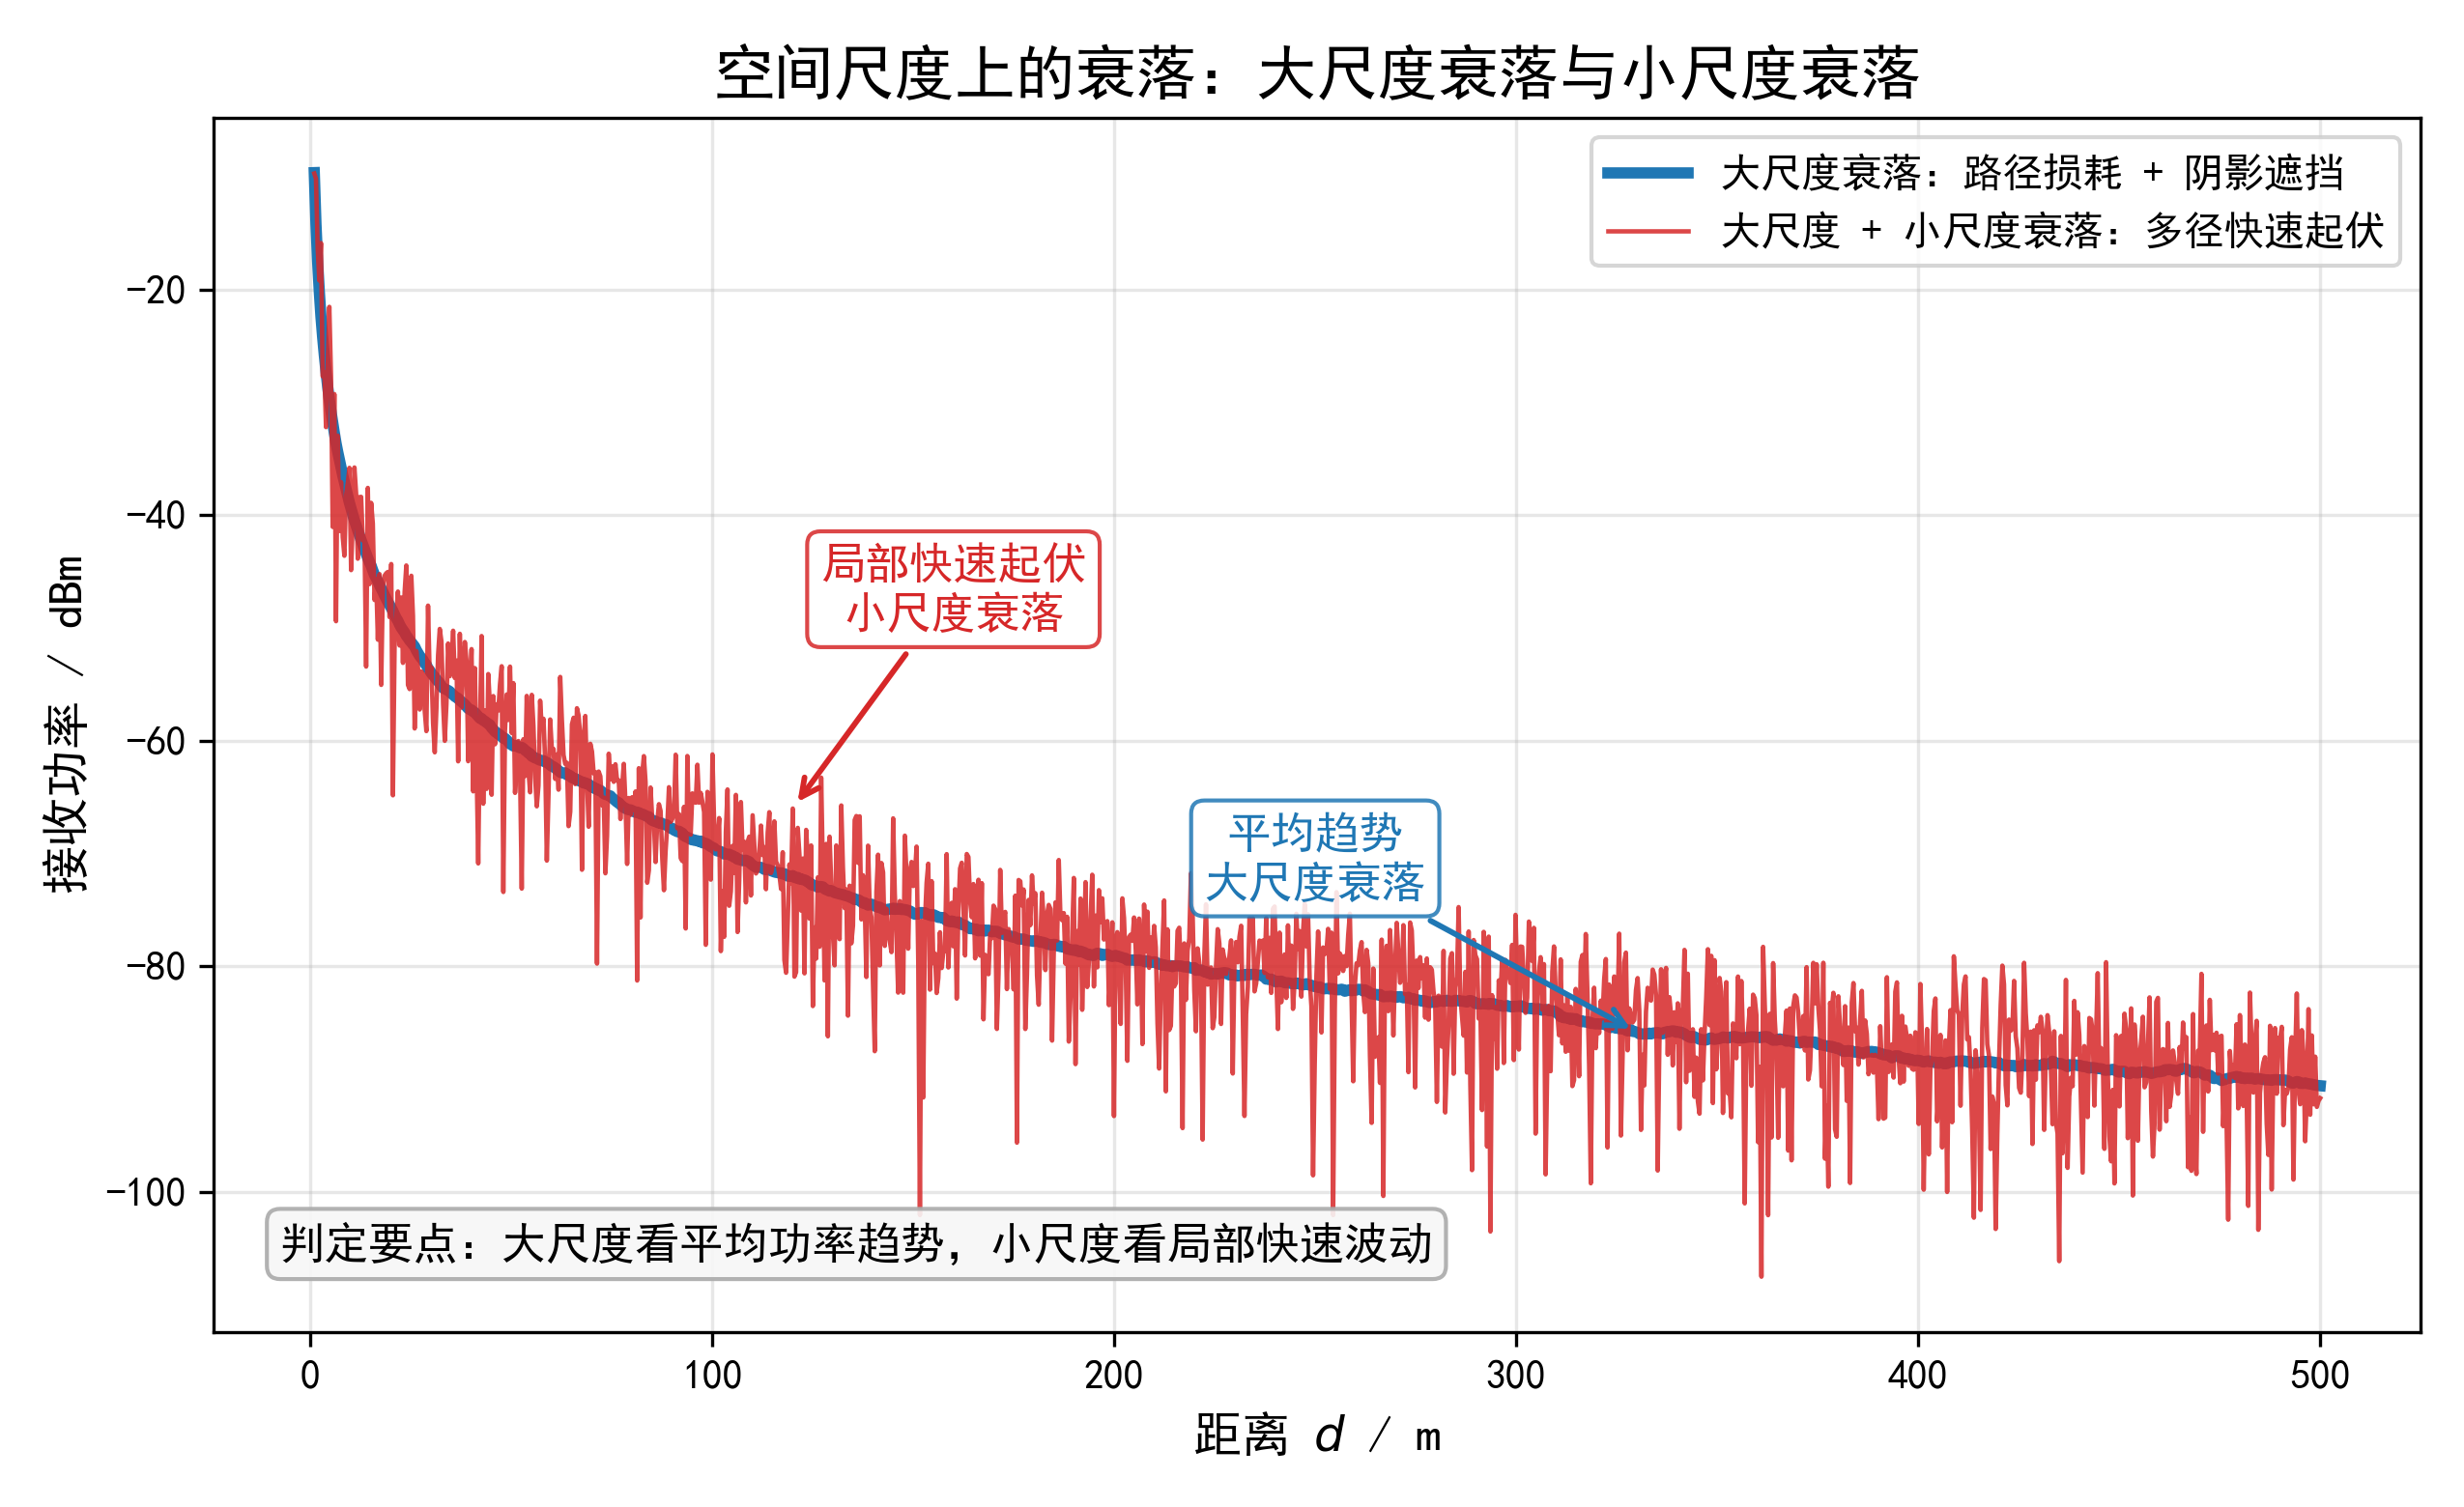
\includegraphics[width=0.75\textwidth]{figures/chapter1/fig_fading.png}
    \caption{大尺度衰落与小尺度衰落对比图}
    \label{fig:spatial-fading}
\end{figure}
\noindent\textbullet\quad\textbf{从时间维度看：多普勒频移、相干时间与快慢衰落}

从时间维度看，
衰落与信道的时变特性密切相关。
当发射端、接收端或环境中的散射体存在相对运动时，
各传播路径上的幅度和相位可能随时间发生变化，
从而使信道呈现非平稳或时变特性。
其中，
由相对运动引起的相位变化会表现为多普勒频移。
最大多普勒频移通常可以写为
\begin{equation}
    f_D
    =
    \frac{v}{\lambda}
    =
    \frac{v f_c}{c},
    \label{eq:maximum-doppler-shift}
\end{equation}
其中，
\(v\) 表示相对速度，
\(\lambda\) 表示载波波长，
\(f_c\) 表示载波频率，
\(c\) 表示光速。
由式~\eqref{eq:maximum-doppler-shift} 可以看出，
在相同载波频率下，
相对速度越高，
多普勒频移越大；
在相同运动速度下，
载波频率越高、波长越短，
多普勒效应也越明显。
因此，
高速移动场景和毫米波、太赫兹等高频通信场景中，
信道随时间变化的问题更加突出。

为了描述信道在时间上的稳定程度，
通常引入\textbf{相干时间} \(T_c\) 的概念。
相干时间可以理解为信道在时间上近似保持不变的时间尺度。
一般而言，
相干时间与最大多普勒频移近似成反比，
即
\begin{equation}
    T_c
    \propto
    \frac{1}{f_D}.
    \label{eq:coherence-time}
\end{equation}
多普勒频移越大，
相干时间越短，
说明信道变化越快；
多普勒频移越小，
相干时间越长，
说明信道在较长时间内更加稳定。

在此基础上，
可以理解慢衰落和快衰落的区别。
设信号的符号持续时间为 \(T_s\)。

\textbf{慢衰落}是指信道变化相对于信号变化较慢的情形。
如果 \(T_s \ll T_c\)，
则在一个符号周期内信道基本保持不变，
接收信号可以近似看作经过一个相对固定的信道传输。
这种情况下，
信道变化主要体现在较长时间尺度上，
通常称为慢衰落。

\textbf{快衰落}是指信道变化相对于信号变化较快的情形。
如果 \(T_s\) 与 \(T_c\) 接近，
甚至大于 \(T_c\)，
则信道可能在一个符号周期内发生明显变化，
从而使接收信号在符号内部也经历时变信道影响。
这种情况下，
接收端的同步、信道估计和均衡会更加困难，
通常称为快衰落。

因此，
快衰落和慢衰落并不是单纯由“移动速度快不快”决定的绝对概念，
而是由信道变化时间尺度与信号时间尺度之间的相对关系决定的。

\noindent\textbullet\quad\textbf{从频率维度看：时延扩展、相干带宽与频率选择性}

从频率维度看，
衰落与多径时延扩展密切相关。
在多径传播中，
不同路径具有不同的传播距离，
因此到达接收端的时间并不完全相同。
多个路径分量在时延轴上分散开来的现象称为时延扩展。
常用均方根时延扩展 \(\tau_{\mathrm{rms}}\)
描述多径能量在时延轴上的分散程度。
时延扩展越大，
说明不同多径分量之间的到达时间差越明显，
信道频率响应随频率变化的起伏通常也越强。

为了描述信道在频率上的相关范围，
通常引入\textbf{相干带宽} \(B_c\) 的概念。
相干带宽可以理解为信道频率响应在频率上近似保持一致的频率范围。
一般而言，
相干带宽与均方根时延扩展近似成反比，
即
\begin{equation}
    B_c
    \propto
    \frac{1}{\tau_{\mathrm{rms}}}.
    \label{eq:coherence-bandwidth}
\end{equation}
时延扩展越大，
相干带宽越小，
说明信道在较窄的频率范围内就可能发生明显变化；
时延扩展越小，
相干带宽越大，
说明较宽频带内的信道响应仍可能比较相似。

\textbf{平坦衰落}是指信号带宽 \(B\)
远小于相干带宽 \(B_c\) 时的衰落形式，
即 \(B \ll B_c\)。
在这种情况下，
信号带宽内的各个频率分量经历近似相同的信道响应，
整个信号频带可以近似看作受到同一个复数信道系数的影响。
因此，
平坦衰落虽然会改变信号的整体幅度和相位，
但通常不会使不同频率分量产生明显不同的失真。

\textbf{频率选择性衰落}是指信号带宽 \(B\)
与相干带宽 \(B_c\) 接近，
或者 \(B > B_c\) 时的衰落形式。
在这种情况下，
不同频率分量可能经历不同的幅度衰减和相位变化，
因此接收信号会出现频域上的非均匀失真。
频率选择性衰落是宽带无线通信中的重要问题，
也是 OFDM 多载波传输技术的重要动机之一。
OFDM 通过将宽带信号划分为多个窄带子载波，
使每个子载波上的信道近似表现为平坦衰落信道，
从而降低均衡和接收处理的复杂度。

需要强调的是，
大尺度衰落、小尺度衰落、慢衰落、快衰落、
平坦衰落和频率选择性衰落并不是彼此互斥的分类。
它们只是从不同观察角度描述无线信道的变化特性：
空间尺度关注接收信号随位置变化的趋势，
时间维度关注信道随时间变化的快慢，
频率维度关注信道对不同频率分量的不同影响。
一个实际无线信道可能同时受到路径损耗、阴影遮挡、多径叠加、
移动性和频率选择性等因素的影响。

对于传统通信系统而言，
衰落主要体现为影响可靠传输和链路质量的不利因素；
而对于 ISAC 系统而言，
衰落背后的时延、多普勒、角度和路径增益等物理量，
也可能携带目标运动、空间结构和环境状态等感知信息。
因此，
在 ISAC 中理解衰落不仅是为了补偿信道影响，
也是为了进一步利用无线传播过程中的环境信息。

上述衰落概念分别从空间尺度、时间变化和频率响应等角度描述无线信道的不同特性。
为了便于对比和记忆，
表~\ref{tab:fading-types-comparison} 对常见衰落类型的主要来源、
判定要素和直观含义进行了总结。
在实际无线环境中，
这些衰落现象往往会同时存在，
共同影响通信链路质量和 ISAC 系统的感知性能。
\begin{table}[htbp]
    \centering
    \caption{不同衰落类型的对比}
    \label{tab:fading-types-comparison}
    \renewcommand{\arraystretch}{1.35}
    \begin{tabularx}{\textwidth}{p{0.13\textwidth} p{0.16\textwidth} X X X}
        \hline
        \textbf{观察维度}
        &
        \textbf{衰落类型}
        &
        \textbf{主要来源}
        &
        \textbf{判定要素}
        &
        \textbf{直观理解}
        \\
        \hline

        空间尺度
        &
        大尺度衰落
        &
        路径损耗、阴影遮挡、地形与建筑物阻挡
        &
        接收信号平均功率随位置或距离缓慢变化
        &
        信号整体变弱或被遮挡
        \\

        空间尺度
        &
        小尺度衰落
        &
        多径分量的相干叠加
        &
        接收信号在短距离或短时间内快速起伏
        &
        移动很短距离，信号也可能明显增强或减弱
        \\

        时间维度
        &
        慢衰落
        &
        低移动性、较小多普勒频移
        &
        \(T_s \ll T_c\)
        &
        一个符号周期内信道近似不变
        \\

        时间维度
        &
        快衰落
        &
        高移动性、较大多普勒频移或快速变化的散射环境
        &
        \(T_s \gtrsim T_c\)
        &
        一个符号周期内信道已经明显变化
        \\

        频率维度
        &
        平坦衰落
        &
        较小的多径时延扩展
        &
        \(B \ll B_c\)
        &
        整个信号带宽内的频率分量经历近似相同的信道
        \\

        频率维度
        &
        频率选择性衰落
        &
        较大的多径时延扩展
        &
        \(B \gtrsim B_c\)
        &
        不同频率分量经历不同幅度衰减和相位变化
        \\
        \hline
    \end{tabularx}
\end{table}


\paragraph{通信质量指标分类}

前面讨论的路径损耗、多径传播、衰落、噪声和干扰，
都会改变接收端观测到的信号质量。
为了评价这些因素对信息传输的影响，
通信系统需要引入一系列质量指标。
不同指标关注的层面并不相同：
有些指标描述接收信号本身的质量，
有些指标衡量信息恢复是否可靠，
还有一些指标反映系统在有限频谱和时间资源下能够传输多少有效信息。
因此，
通信质量指标可以大致分为三类：
\textbf{链路质量指标}、\textbf{可靠性指标}和\textbf{效率指标}。

\textbf{链路质量指标}主要用于描述接收端有用信号相对于噪声或干扰的强弱关系，
典型指标包括信噪比（signal-to-noise ratio, SNR）
和信干噪比（signal-to-interference-plus-noise ratio, SINR）。
信噪比定义为有用信号功率与噪声功率之比，
即
\begin{equation}
    \mathrm{SNR}
    =
    \frac{P_s}{P_n},
    \label{eq:snr-definition}
\end{equation}
其中，
\(P_s\) 表示接收端的有用信号功率，
\(P_n\) 表示噪声功率。
若噪声功率谱密度为 \(N_0\)，
系统带宽为 \(B\)，
则噪声功率常可写为
\begin{equation}
    P_n
    =
    N_0 B.
    \label{eq:noise-power-bandwidth}
\end{equation}
因此，
在接收信号功率固定的情况下，
带宽增大会引入更多噪声功率，
从而可能降低 SNR。
一般来说，
发射功率越高、路径损耗越小、
天线增益或波束增益越大，
接收信号功率越强，
SNR 越高；
而噪声功率越大，
SNR 越低。

在实际系统中，
接收端受到的非期望成分往往不只有噪声，
还包括来自其他用户、邻近小区、同频系统或共享频谱设备的干扰。
因此，
信干噪比比 SNR 更适合描述实际通信链路质量，
其定义为
\begin{equation}
    \mathrm{SINR}
    =
    \frac{P_s}{P_i + P_n},
    \label{eq:sinr-definition}
\end{equation}
其中，
\(P_i\) 表示干扰功率。
当干扰功率较小时，
SINR 近似退化为 SNR；
当系统处于干扰受限状态时，
即使提高发射功率，
通信性能也可能提升有限，
此时干扰协调、资源调度、功率控制和波束成形等技术会变得更加重要。
对于 ISAC 系统而言，
SINR 的意义更加突出，
因为通信与感知功能可能共享时间、频率、空间和功率资源，
通信信号、感知回波、杂波以及其他用户信号之间
可能形成更加复杂的相互影响。

\textbf{可靠性指标}用于衡量接收端能否正确恢复发送端的信息。
最常见的可靠性指标是误码率（bit error rate, BER），
其定义为错误比特数与总传输比特数之比：
\begin{equation}
    \mathrm{BER}
    =
    \frac{N_{\mathrm{error}}}{N_{\mathrm{total}}},
    \label{eq:ber-definition}
\end{equation}
其中，
\(N_{\mathrm{error}}\) 表示接收端判决错误的比特数，
\(N_{\mathrm{total}}\) 表示总传输比特数。
BER 越低，
说明通信链路的可靠性越高。
通常情况下，
SNR 或 SINR 越高，
接收端越容易区分不同调制符号，
BER 越低；
而当衰落严重、干扰增强或噪声功率增大时，
BER 往往会上升。

误码率还与调制方式和信道编码密切相关。
在相同 SNR 条件下，
高阶调制方式能够在每个符号中携带更多比特，
但星座点之间的距离更近，
因此通常更容易受到噪声和干扰影响；
低阶调制方式虽然频谱效率较低，
但鲁棒性更强。
信道编码可以通过引入冗余帮助接收端检测和纠正错误，
从而降低误码率，
但也会带来一定的速率开销。
在实际移动通信系统中，
还常使用块错误率（block error rate, BLER）
描述一个传输块是否被正确解码。
相比 BER，
BLER 更接近链路自适应、重传机制和实际吞吐率的评价需求。

\textbf{效率指标}用于衡量通信系统在有限资源下传输信息的能力。
最基本的速率指标是数据率，
表示单位时间内传输的信息比特数。
在理想高斯信道中，
信道容量可以作为理论上限参考，
其形式为
\begin{equation}
    C
    =
    B \log_2
    \left(
        1+\mathrm{SNR}
    \right),
    \label{eq:capacity-snr}
\end{equation}
其中，
\(C\) 表示信道容量，
\(B\) 表示系统带宽。
如果考虑干扰影响，
也常将 SNR 替换为 SINR，
写作
\begin{equation}
    C
    =
    B \log_2
    \left(
        1+\mathrm{SINR}
    \right).
    \label{eq:capacity-sinr}
\end{equation}
式~\eqref{eq:capacity-snr} 和式~\eqref{eq:capacity-sinr} 表明，
容量与带宽和链路质量都有关。
增大带宽可以提供更多频率资源，
提高 SNR 或 SINR 可以提升单位带宽内可承载的信息量。
但是，
容量随 SNR 或 SINR 的增长呈对数关系，
因此在高信噪比区域，
继续提高功率带来的速率增益会逐渐减小。

吞吐率更接近实际系统中成功传输的信息量。
它可以理解为单位时间内被接收端正确接收的有效数据量，
常写为
\begin{equation}
    R_{\mathrm{throughput}}
    =
    \frac{N_{\mathrm{success}}}{T},
    \label{eq:throughput-definition}
\end{equation}
其中，
\(N_{\mathrm{success}}\) 表示在时间 \(T\) 内成功接收的信息比特数。
若用 \(R\) 表示名义传输速率，
用 BLER 表示块错误率，
则实际吞吐率可近似表示为
\begin{equation}
    R_{\mathrm{throughput}}
    \approx
    R
    \left(
        1-\mathrm{BLER}
    \right).
    \label{eq:throughput-bler}
\end{equation}
这一表达式说明，
较高的名义速率并不一定意味着较高的实际吞吐率。
如果信道条件较差，
导致错误率或重传概率升高，
实际成功传输的数据量可能反而下降。

频谱效率（spectral efficiency）用于衡量单位带宽内能够传输多少信息，
通常定义为
\begin{equation}
    \eta
    =
    \frac{R}{B},
    \label{eq:spectral-efficiency-definition}
\end{equation}
单位为 bit/s/Hz。
如果以信道容量作为理想参考，
则频谱效率可以写为
\begin{equation}
    \eta
    =
    \log_2
    \left(
        1+\mathrm{SNR}
    \right),
    \label{eq:spectral-efficiency-snr}
\end{equation}
或者在考虑干扰时写为
\begin{equation}
    \eta
    =
    \log_2
    \left(
        1+\mathrm{SINR}
    \right).
    \label{eq:spectral-efficiency-sinr}
\end{equation}
频谱效率越高，
说明系统在有限频谱资源中传输信息的能力越强。
在频谱资源日益紧张的背景下，
频谱效率是评价无线通信系统的重要指标之一。
对于 ISAC 而言，
频谱效率还具有更特殊的意义：
ISAC 希望通过通信与感知共享频谱、硬件和波形资源，
在不额外占用大量频谱的情况下同时支持信息传输和环境感知。
因此，
频谱效率不仅反映通信链路本身的资源利用能力，
也与通感资源复用和系统整体效率密切相关。

在实际系统中，
这些通信质量指标之间存在清晰的逻辑关系。
路径损耗、多径、衰落、噪声和干扰
首先影响接收端的 SNR 或 SINR；
SNR 或 SINR 进一步决定解调和译码的可靠性，
并体现在 BER 或 BLER 等指标上；
可靠性又会影响实际吞吐率，
而在给定带宽下，
有效传输速率进一步决定频谱效率。
因此，
可以将通信质量指标理解为从“接收信号质量”到“信息恢复可靠性”，
再到“资源利用效率”的逐层度量。
对于 ISAC 系统而言，
这些指标仍然是评价通信性能的基础，
同时也为后续讨论通信与感知之间的性能权衡、
资源分配和联合优化提供了重要依据。

\paragraph{信道状态信息的定义、获取与作用}

通信系统若要根据无线信道状态进行接收处理和传输优化，
首先需要获得对当前信道的描述信息，
这类信息通常称为\textbf{信道状态信息}
（channel state information, CSI）。
CSI 反映了信号在传播过程中受到的幅度衰减、
相位旋转、时延扩展、频率选择性以及空间方向等影响。
换言之，
CSI 可以看作通信系统对无线信道当前状态的数学描述。

CSI 的具体形式与系统结构有关。
在单天线窄带系统中，
CSI 可以简化为一个复数信道系数
\begin{equation}
    h
    =
    |h|e^{j\phi},
    \label{eq:csi-siso-coefficient}
\end{equation}
其中，
\(|h|\) 描述信号幅度的变化，
\(\phi\) 描述信号相位的变化。
在 OFDM 系统中，
CSI 通常表示为不同子载波上的频域信道响应
\begin{equation}
    H[k],
    \label{eq:csi-ofdm-subcarrier}
\end{equation}
其中，
\(k\) 表示子载波索引，
\(H[k]\) 描述第 \(k\) 个子载波上的信道幅度和相位变化。
在 MIMO 系统中，
CSI 则常表示为信道矩阵
\begin{equation}
    \mathbf{H},
    \label{eq:csi-mimo-matrix}
\end{equation}
其矩阵元素描述不同发射天线与接收天线之间的空间信道关系。
由此可见，
CSI 并不固定为某一种形式，
但其核心作用都是描述无线信道对发射信号的影响。

CSI 通常通过导频或参考信号进行估计。
发送端在预定的时间、频率或空间资源位置发送接收端已知的导频符号，
接收端根据导频的已知发送值和对应接收值估计信道。
在不同系统和假设条件下，
可以采用不同的信道估计算法，
例如最小二乘估计（least squares, LS）、
线性最小均方误差估计
（linear minimum mean square error, LMMSE）
以及结合插值、滤波或压缩感知的方法。
在 OFDM 系统中，
CSI 往往需要在多个导频子载波上获得，
再通过频域或时域插值估计其他资源位置上的信道响应；
在 MIMO 系统中，
还需要估计不同发射天线和接收天线之间的信道矩阵。

CSI 的获取方式还与双工方式有关。
在 FDD 系统中，
上行和下行通常使用不同频段，
二者信道不完全相同，
因此接收端估计下行 CSI 后，
通常需要通过反馈链路将信道质量或预编码相关信息反馈给发射端。
在 TDD 系统中，
上行和下行使用同一频段的不同时隙，
理想情况下无线传播信道具有互易性，
因此基站可以根据上行导频估计信道，
并将其用于下行传输设计。
不过，
在实际系统中，
信道互易性还会受到射频前端差异的影响，
因此通常需要进行一定的校准。

CSI 在通信系统设计中具有基础作用。
首先，
接收端可以利用 CSI 进行信道均衡，
补偿信道引起的幅度衰减、相位旋转和频率选择性失真，
从而提高解调和译码的可靠性。
其次，
发射端或系统调度器可以根据信道质量进行自适应调制编码：
当信道条件较好时，
可以采用高阶调制和较高编码率以提升速率；
当信道条件较差时，
则可以采用低阶调制和更强的信道编码以保证可靠性。
此外，
CSI 还可以用于功率控制、用户调度、资源分配以及重传策略设计。

在 MIMO 系统中，
CSI 的作用更加突出。
发射端或接收端可以根据信道矩阵设计波束成形和预编码权重，
使发射能量尽可能集中到目标用户方向，
同时抑制对其他用户的干扰。
对于多用户 MIMO 系统，
CSI 还可以帮助系统判断哪些用户适合在同一时频资源上进行空间复用，
从而提高系统容量和频谱效率。
可以说，
CSI 是通信系统从固定传输走向自适应传输的重要基础。

从 ISAC 的角度看，
CSI 的意义进一步扩展。
在传统通信系统中，
CSI 主要用于补偿信道影响、
提高通信可靠性和传输效率；
而在 ISAC 系统中，
CSI 本身也可能包含目标和环境信息。
例如，
信道中的时延信息可能对应传播路径长度或目标距离，
多普勒频移可能反映目标或散射体的相对运动，
角度信息可能对应目标方向或空间结构，
路径增益和反射特性则可能反映目标散射强度或环境材料特征。
因此，
CSI 不仅是通信链路自适应设计的依据，
也可能成为 ISAC 系统感知环境和理解目标状态的重要入口。

由此可以看出，
CSI 将无线信道的物理特性与通信系统设计连接起来。
对于通信而言，
CSI 用于适应和补偿信道；
对于 ISAC 而言，
CSI 还可以帮助系统从信道变化中提取环境、目标和运动信息。
这也是后续讨论 OFDM 信道估计、MIMO 波束成形
以及通信-感知联合处理时需要反复依赖的基础概念。